% % ###########################
% \tikzexternalenable
% % ###########################
\subsection{Input Data Format}
\begin{algorithm}[!t]
    \SetAlgoLined
    \LinesNumbered
    
    \SetKwFunction{Dictionary}{Dictionary}
    \SetKwFunction{List}{List}
    \SetKwInOut{Input}{input}
    \SetKwInOut{Output}{output}
    
    \Input{Dataset, TargetDiseaseGroup, DiseaseGroups}
    \Output{Encoding} 
    \BlankLine
    Encoding $\leftarrow$ new  \Dictionary{}\;
    \For{$diseaseGroup \in DiseaseGroups$}{
        Encoding[diseaseGroup][patientID] $\leftarrow$ new \List{}\;
        Encoding[diseaseGroup][gender] $\leftarrow$ new \List{}\;
        Encoding[diseaseGroup][record] $\leftarrow$ new \List{}\;
        Encoding[diseaseGroup][target] $\leftarrow$ new \List{}\;
        \For{$record \in Dataset$}{
            \emph{//encode Dataset into a weekly trinary sequence}\;
            weeklyEncoding $\leftarrow$ new \List{}\;
            \For{$weeklyDiseaseRecord \in record$}{
                \emph{//no code recorded for the observed week}\;
                \If{$weeklyDiseaseRecord.code == NIL$}{
                    append "0" to weeklyEncoding\;
                }
                \If{$weeklyDiseaseRecord.code \in diseaseGroup.codes$}{
                    append "1" to weeklyEncoding\;
                }
                \If{$weeklyDiseaseRecord.code \notin diseaseGroup.codes$}{
                    append "2" to weeklyEncoding\;
                }
            }
            target $\leftarrow$ 1 if any weeklyDiseaseRecord.code of record $\in$ TargetDiseaseGroup\;
            \If{$target == 1$}{
                cut weeklyEncoding up to (but not including) first occurrence of TargetDiseaseGroup member\;
            }
            append record.patientID to Encoding[diseaseGroup][patientID]\;
            append record.gender to Encoding[diseaseGroup][gender]\;
            append weeklyEncoding to Encoding[diseaseGroup][record]\;
            append target to Encoding[diseaseGroup][target]\;
        }
    }
    \Return{Encoding}\;
    \caption{ICD-9 Encoding}\label{algo1}
\end{algorithm}


\begin{algorithm}[!t]
    \SetAlgoLined
    \LinesNumbered
    
    \SetKwFunction{Dictionary}{Dictionary}
    \SetKwFunction{List}{List}
    \SetKwFunction{Dataframe}{Dataframe}
    \SetKwFunction{TrainTestSplit}{TrainTestSplit}
    \SetKwFunction{genESeSS}{genESeSS}
    \SetKwFunction{ComputeSequenceFeature}{ComputeSequenceFeature}
    \SetKwFunction{llk}{llk}
    \SetKwFunction{pairwise}{pairwise}
    \SetKwFunction{outerjoin}{outerjoin}
    \SetKwFunction{LightGBM}{LightGBM}
    
    \SetKwInOut{Input}{input}
    \SetKwInOut{Output}{output}
    
    \Input{Encoding, DiseaseGroups, SequenceFeatures, hyperparameters}
    \Output{Predictions, FeatureImportances} 
    \BlankLine
    DiseaseDatasets $\leftarrow$ new  \Dictionary{}\;
    \For{$Dataset, DiseaseGroup \in zip(Encoding, DiseaseGroups)$}{
        PFSAset, LLset $\leftarrow$ \TrainTestSplit{Dataset, w.r.t = "target"}\;
        df $\leftarrow$ new \Dataframe{}\;
        df[patientID] $\leftarrow$ LLset[patientID]\;
        df[target] $\leftarrow$ LLset[target]\;
        \emph{//Generate 2 PFSAs for each class}\;
        PositivePFSAset $\leftarrow$ PFSAset[PFSAset.target == 1]\;
        NegativePFSAset $\leftarrow$ PFSAset[PFSAset.target == 0]\;
        PosPFSA $\leftarrow$ \genESeSS{PositivePFSAset}\;
        NegPFSA $\leftarrow$ \genESeSS{NegativePFSAset}\;
        \emph{//For each record, compute loglikelihoods of being generated by either of 2 PFSAs generated above}\;
        PosLLK $\leftarrow$ \llk{LLset, PosPFSA}\;
        NegLLK $\leftarrow$ \llk{LLset, NegPFSA}\;
        \emph{//Compute sequence likelihood defect}\;
        df[DiseaseGroup] $\leftarrow$ \pairwise{PosLLK - NegLLK}\;
        df[DiseaseGroup + '\_abs\_neg'] $\leftarrow$ NegLLK\;
        \For{$SequenceFeature \in SequenceFeatures$} { 
            df[DiseaseGroup + '\_' +  SequenceFeature] $\leftarrow$ [\ComputeSequenceFeature{SequenceFeature, seq} for each seq $\in$ LLset['record']]\;
        }
        DiseaseDatasets[DiseaseGroup] $\leftarrow$ df\;
    }
    Dataset $\leftarrow$ \outerjoin{DiseaseDatasets.values, on = 'patientID'}\;
    Aggregate all features in Dataset where feature\_name $\in$ DiseaseGroups (mean, std. deviation, range)\;
    Aggregate all features in Dataset where feature name minus '\_abs\_neg' $\in$ DiseaseGroups (mean, std. deviation, range)\;
    Aggregate all sequence features in Dataset (mean, std. deviation, range, max)\;
    TrainSet, TestSet $\leftarrow$ \TrainTestSplit{Dataset, w.r.t = "target"}\;
    LGBM $\leftarrow$ new \LightGBM{hyperparameters}\;
    LGBM.fit(TrainSet)\;
    Predictions $\leftarrow$ LGBM.predict(TestSet)\;
    \Return{Predictions, LGBM.feature\_importances}\;
    \caption{Prediction Pipeline Training}\label{algo2}
\end{algorithm}
% \begin{figure}[!ht]
%   \centering
  
%   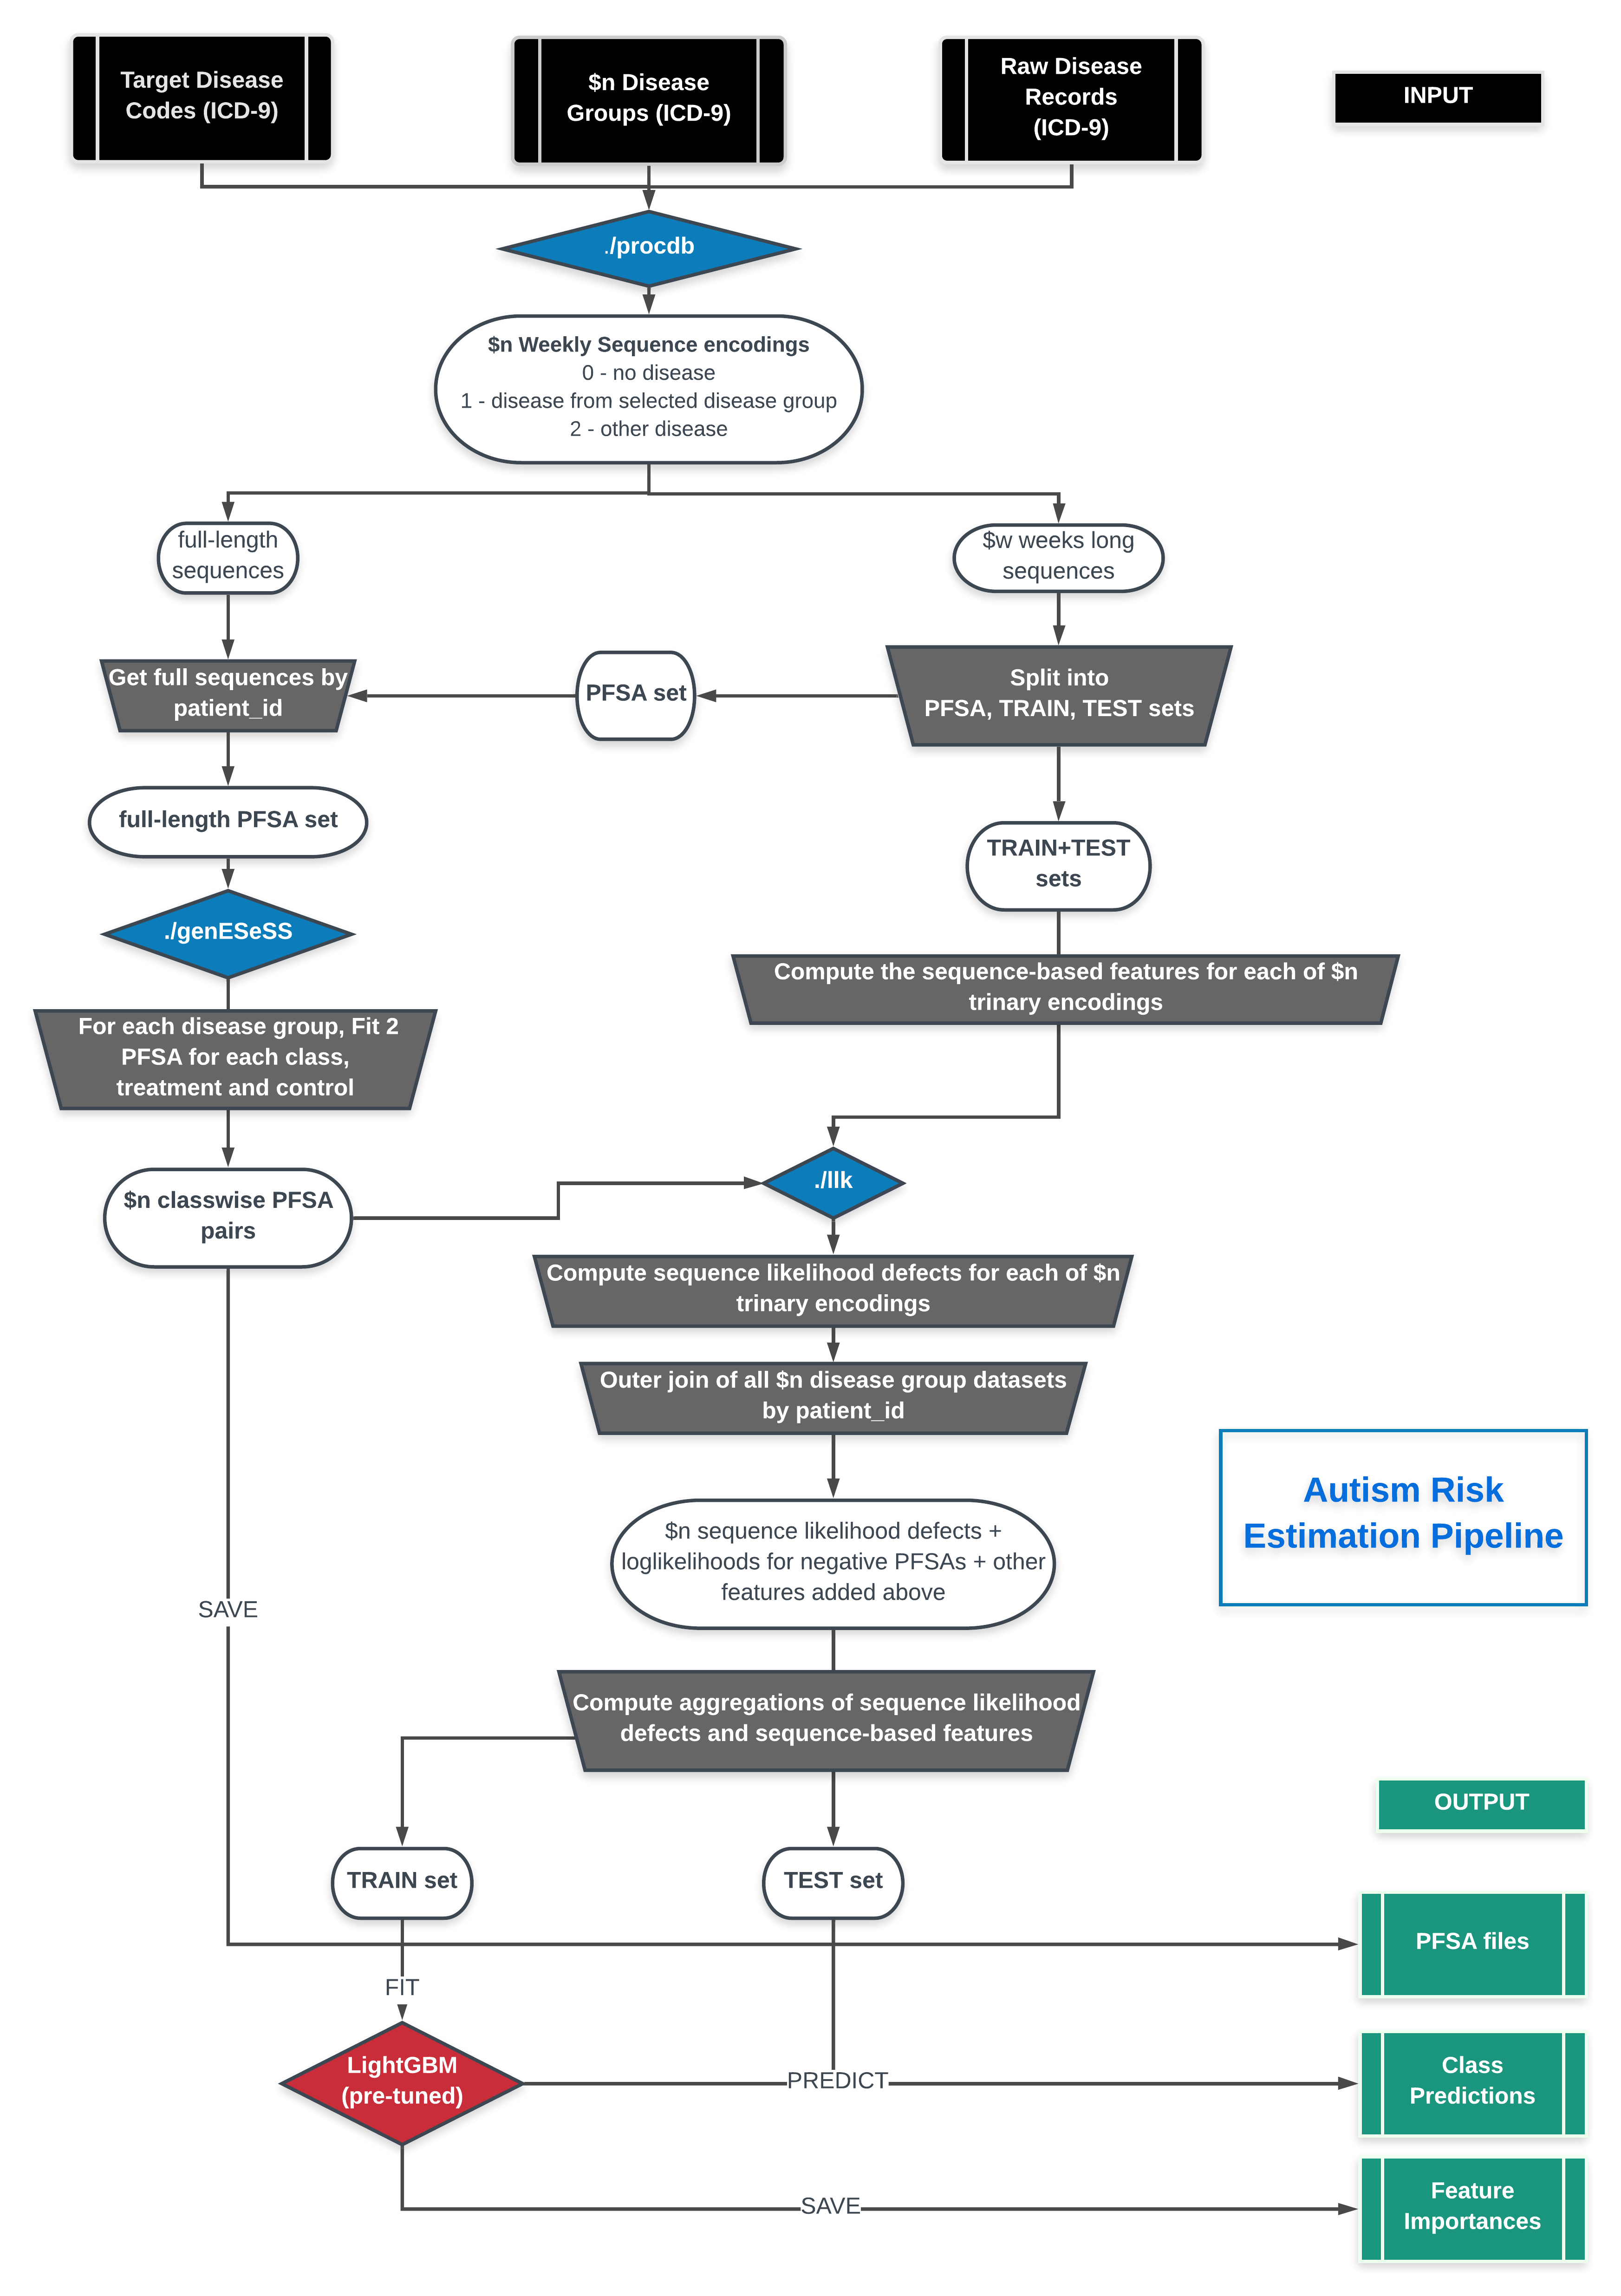
\includegraphics[width=\textwidth]{Figures/Pipeline}
%   \captionN{Pipeline schema: How the data set is split into test sets and two training sets: one for inferring HMM models, and one for training the boosting classifier.}\label{figschema}
%   \vspace{-20pt}
% \end{figure}


% Individual weekly medical history records, for a large cohort of US children between the years 2003 and 2010. The data is an excerpt from an insurance claims database tracking over 200 million people in US over a decade, with ICD-9 code representation of diseases. Each medical record is a list of ICD-9 codes with recorded week disease occurred.
% Records are classified by patient’s gender and county (FIPS code) of residence. The following pipeline works with two gender subsets of the input data separately.

To encode the ICD-9 codes, 17 Disease Groups of codes are used  to transform the raw health records into a format suitable for PFSA. As described in $Algorithm 1$, for each patient, the list of ICD-9 codes is encoded into a weekly array of three-symbol alphabet digits with respect to selected disease group, for each week: "0" - no disease "1" - disease from the selected group, "2" - other disease.

Once the trinary encodings are ready, the PFSA pairs are fit for each of the disease groups, on positive (treatment) and negative (control) sets using \texttt{genESeSS} algorithm~\cite{CL12g} (See Section~\ref{sec:PFSA}), as described in $Algorithm$ $2$. The PFSA pairs are then used to obtain the loglikelihood scores of belonging to a  PFSA modeling the positive and the control cohorts accordingly for each of the encodings of a patient record. As a result, we yield the difference between positive and control loglikelihoods for each disease group of each patient. The positive value of difference means that with respect to a given disease group, a certain patient is more likely to be a positive one. Conversely, the negative value of difference signifies that a patient is more likely to be from the control group. These features, as well as their aggregations and the aggregations of the ternary encoding arrays, are used as the features for the final  LightGBM gradient boosting classifier.

% \\
%%%%%%%%%%%%%%%%%%%%%%%%%%%%%%%%%%%%%%%%%%%%%%%%%%%%%%%%%%%%%%
\subsection{Algorithms}
The key data processing approach is outlined in Algorithm~\ref{algo1}. The remaining steps of the approach are sketched in Algorithm~\ref{algo2}. Fig.~\ref{figschema} shows the overall schema, including the breakdown of a database into a test set, and two training sets: one for training the HMM models, and one for training the boosting classifier.

\begin{figure}[!ht]
  \centering
  
  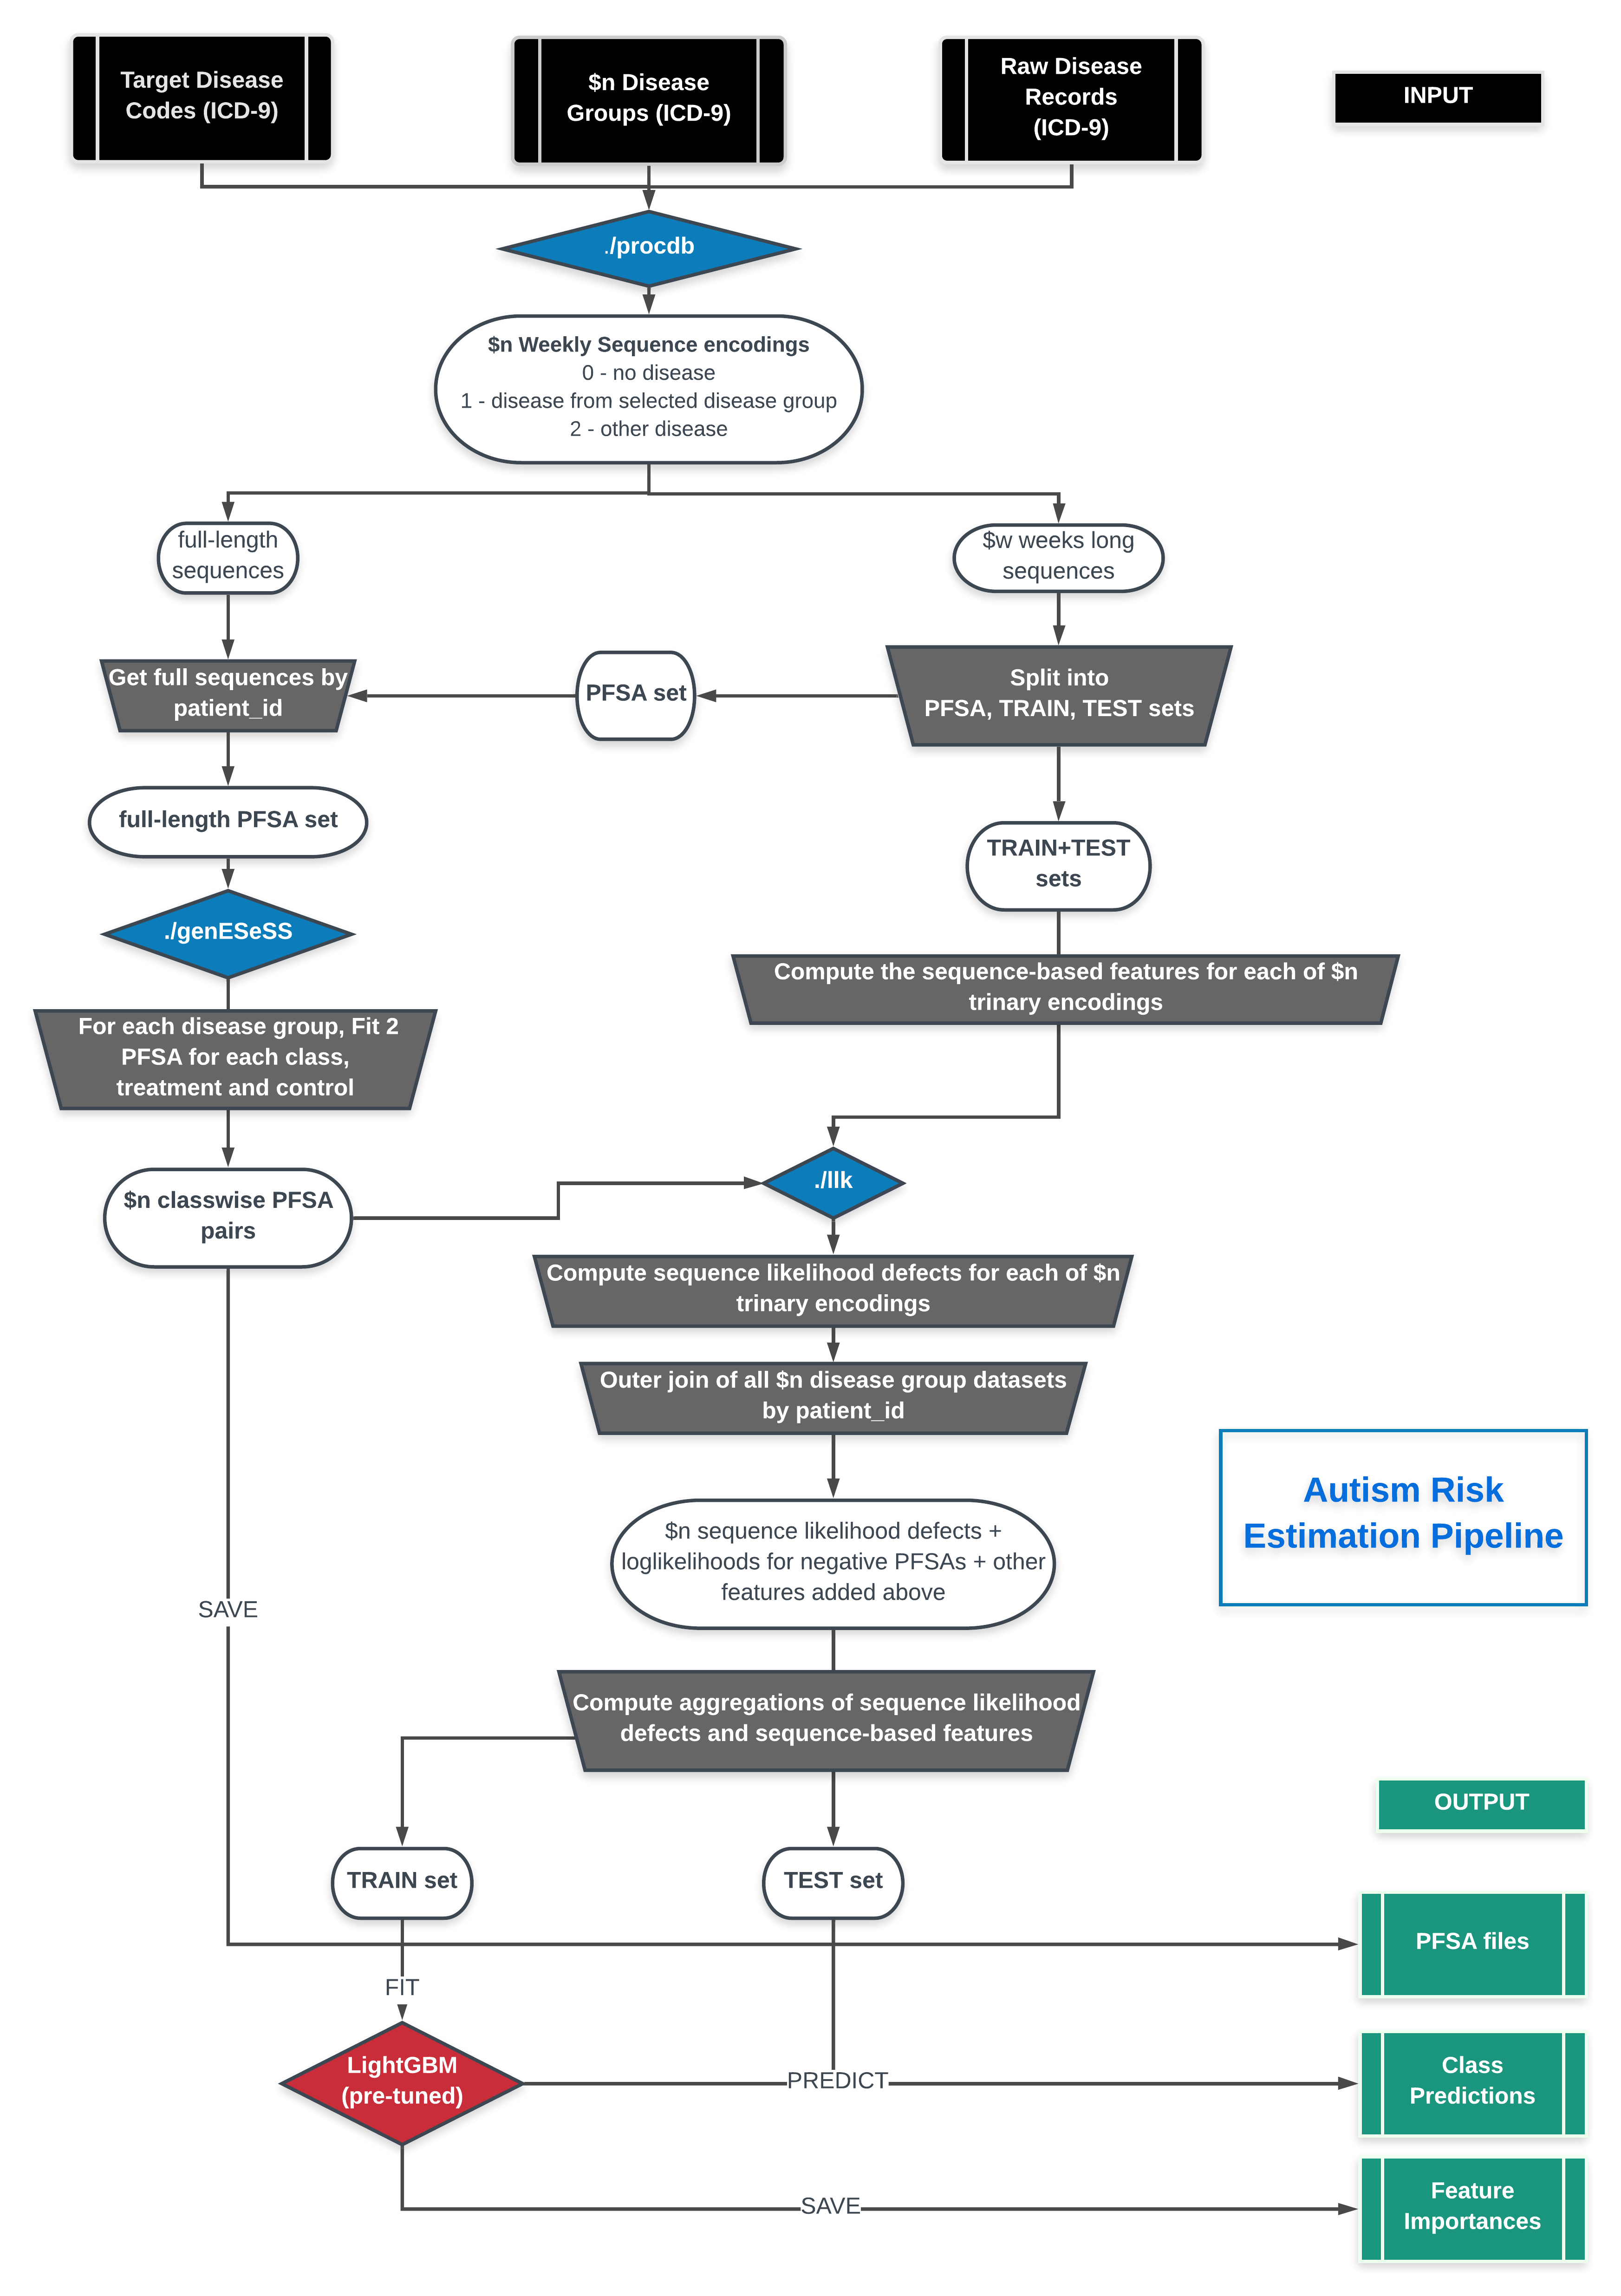
\includegraphics[width=.85\textwidth]{Figures/Pipeline}
  \captionN{Pipeline schema: How the data set is split into test sets and two training sets: one for inferring HMM models, and one for training the boosting classifier. The two key algorithms here are \texttt{genESeSS}~\cite{CL12g} and the llk which does the sequence likelihood computation described in Section~\ref{sec:SLD}}\label{figschema}
  \vspace{-20pt}
\end{figure}